\documentclass[a4paper, 10pt, american]{article}
\usepackage[utf8]{inputenc}
\usepackage{csquotes}
\usepackage{bookmark}
\usepackage{hyperref}
\usepackage[american]{babel}
\usepackage[margin=1in]{geometry}
\usepackage{setspace}
\usepackage{multirow}
\usepackage{graphicx}
\usepackage{wrapfig}
\usepackage[inline]{enumitem}
\usepackage{lipsum}
\usepackage{listings}
\usepackage[dvipsnames]{xcolor}
\graphicspath{{./images/}}
\newcommand{\etal}{et~al. }

\hyphenation{smart-phones smart-phone}

\lstdefinelanguage{Kotlin}{
  comment=[l]{//},
  commentstyle={\color{gray}\ttfamily},
  emph={filter, first, firstOrNull, forEach, lazy, map, mapNotNull, println},
  emphstyle={\color{OrangeRed}},
  identifierstyle=\color{black},
  keywords={!in, !is, abstract, actual, annotation, as, as?, break, by, catch, class, companion, const, constructor, continue, crossinline, data, delegate, do, dynamic, else, enum, expect, external, false, field, file, final, finally, for, fun, get, if, import, in, infix, init, inline, inner, interface, internal, is, lateinit, noinline, null, object, open, operator, out, override, package, param, private, property, protected, public, receiveris, reified, return, return@, sealed, set, setparam, super, suspend, tailrec, this, throw, true, try, typealias, typeof, val, var, vararg, when, where, while},
  keywordstyle={\color{NavyBlue}\bfseries},
  morecomment=[s]{/*}{*/},
  morestring=[b]",
  morestring=[s]{"""*}{*"""},
  ndkeywords={@Deprecated, @JvmField, @JvmName, @JvmOverloads, @JvmStatic, @JvmSynthetic, Array, Byte, Double, Float, Int, Integer, Iterable, Long, Runnable, Short, String},
  ndkeywordstyle={\color{BurntOrange}\bfseries},
  sensitive=true,
  stringstyle={\color{ForestGreen}\ttfamily},
}

\title{Thesis Proposal}
\author{Joseph Petitti}
\date{November 17, 2020}

\begin{document}

\begin{titlepage}
\begin{center}
\doublespacing


{\Large \textsc{Appjudicator}: \\
Enhancing Android Network Analysis through UI Monitoring}

\vfill

by \par

Joseph Petitti

\vfill

A Thesis \\
Submitted to the Faculty \\
of the \\
WORCESTER POLYTECHNIC INSTITUTE \\
In partial fulfillment of the requirements for the \\
Degree of Master of Science \\
in \\
Computer Science \par

\vfill

by

\vspace{0.55cm}

\underline{\hspace{3in}} \\

May 2021

\end{center}

\vfill

\begin{flushleft}
APPROVED: \par
\vspace{\baselineskip}

\underline{\hspace{3in}} \\
Professor Craig A. Shue, Major Thesis Advisor \par
\vspace{\baselineskip}

%\underline{\hspace{3in}} \\
%Professor [TBD] Thesis Reader \par
%\vspace{\baselineskip}

\underline{\hspace{3in}} \\
Professor Craig E. Wills, Head of Department \par
\end{flushleft}
\end{titlepage}

\pagenumbering{roman}

\begin{abstract}
	Smartphones are becoming increasingly important in all aspects of life,
	including corporate environments, where ``bring your own device'' (BYOD)
	policies are gaining widespread acceptance. Malware already exists to take
	advantage of Android phones in BYOD settings, aiming to take control of
	devices with access to privileged information by disguising itself as a
	benign app. Malware could be easier to detect if network administrators had
	more insight into employee-owned smartphones. We propose a system, called
	\textsc{Appjudicator}, to address this issue. It implements an accessibility
	service to monitor user interactions with the user interface (UI) of other
	apps, so this context can be used in malware detection. For example, if an
	app sends a new network request without any user interaction, this flow
	could be the result of malware and should be investigated. Our app is a
	host-based software defined networking (SDN) agent that works in conjunction
	with an SDN controller to monitor and control the phone's networking
	abilities based on the organization's SDN rules and our UI context. We build
	a proof of concept application and find that it can successfully combine
	network and UI data with only 10 milliseconds of total added latency in 95\%
	of flows.
\end{abstract}

\clearpage

\section*{Acknowledgments}
\label{sec:acknowledgments}

I would like to express my gratitude to my advisor, Professor Craig Shue, for
guiding me through my graduate education with helpful advice and insightful
feedback. Without his patience and wisdom this thesis could not have happened. I
would also like to thank Yu Liu for his technical help and support throughout
the project, along with Matt Puentes and Cole Granof for their advice and moral
support. I also wish to thank Beckey Schowalter for her help with writing and
grammar. Additionally, I want to express my appreciation to my thesis reader,
Professor Robert Walls, for his helpful feedback on this project. His questions
and criticism, along with those from every member of the WPI Cake Lab, are what
turned this paper from a very rough summary to a polished final product.

\clearpage

\tableofcontents

\clearpage
\pagenumbering{arabic}


\section{Introduction}
\label{sec:introduction}

% Need

Current corporate network administration tools have little insight into the
connections made by employee-owned smartphones, especially in ``Bring Your Own
Device'' (BYOD) scenarios that are becoming increasingly common. It is difficult
for large organizations to maintain security across their networks with such
little knowledge about, and control over, these mobile devices. The fact that
these devices enter and exit the corporate network and connect to other
networks, such their cellular data provider's, on a daily basis complicates this
issue. Smartphones have a wide range of powerful networking and computational
abilities, and are typically privately owned by employees, which raises further
concerns when integrating them into secure network environments.

For example, smartphones have been targeted by malware specifically designed to
infiltrate corporate networks~\cite{kan2016}, such as ``Dresscode'', which
disguises itself as a legitimate app in order to steal data and add infected
devices to a botnet~\cite{palmer2016}. The ``xHelper'' malware can automatically
download and install arbitrary software specified by an attacker, and persists
even after a factory reset~\cite{vijayan2020}. A black market
malware-as-a-service model called Black Rose Lucy even offers control of
infected Android devices to paying customers, potentially giving any malicious
actor an entry point to a secure network~\cite{wong2018}.

If mobile devices are to have access to sensitive corporate network
infrastructure, either from home or from work, administrators need new tools to
monitor and control their network connections. These tools need to be powerful
enough to detect when network connections are made by Trojan horse malware that
is disguised as a benign app, while being still being easy to deploy and manage.
For example, some existing solutions require recompiling Android's kernel or
gaining root access to their device, which is impractical for most users and
exposes them to additional security risks~\cite{google2020}.

% Approach

To solve these issues on Android devices, we propose a new app called
\textsc{Appjudicator} which leverages user interface (UI) interaction and
software-defined networking (SDN) principles to determine whether network flows
are legitimately user-initiated. The app has two components: an accessibility
service that monitors UI interaction and a VPN service that intercepts network
flows and acts as an OpenFlow agent. We use these two sources of information to
correlate network flows with user interaction in a way that is difficult for
malware to evade, since it cannot physically interact with hardware input
devices.

The UI monitoring component will use Android's accessibility API to
asynchronously record physical hardware inputs, such as tapping or swiping the
touch screen. This gives administrators the ability to accurately distinguish
between human-driven and automated network requests.  Meanwhile, the VPN service
acts as an OpenFlow agent and rule cache, giving administrators fine-grained
control over which connections the device is allowed to make. Flows are
augmented with context from the specific device and application, and can be
elevated to the organization's SDN controller if necessary.

% Benefit over cost

Our application provides organizations with a new set of powerful, easy to use
tools for monitoring BYOD Android smartphones in a simple app package that is
easy for users to install. It does not require rooting, recompiling the kernel,
or any other cumbersome processes. It can distinguish between user-generated and
automated network requests with a high degree of confidence using techniques
that are difficult for malware to evade. This makes users safer by detecting
stealthy malware on their devices, and improves the organizations network
security.

The costs of our system include the resource overhead of running the app (CPU
cycles, battery power, etc.) and the cost of installing, running, and
maintaining the controller server. We expect these costs to be a relatively
small addition to existing resources. The app's UI monitoring and VPN service
also add some latency to network requests performed on the phone. In our
experiments \textsc{Appjudicator} added less than 100 milliseconds of total
latency to new TCP connections in 97\% of trials. UDP connections and subsequent
TCP requests to established connections have even less added latency.

% TODO can we justify this latency?

% Competition

Using UI data to distinguish user-initiated behavior and the use of a smartphone
as an SDN agent have been studied by others before, but \textsc{Appjudicator}
combines these aspects in new and important ways. Android host-based SDN agets
have been investigated by Hanguard~\cite{demetriou2017}, and using UI
interaction as context for identifying malicious app behavior was examined in
AppIntent~\cite{yang2013}, but our system combines these approaches to form a
novel solution for a distinct use case. One key difference is that AppIntent
uses machine learning to conduct static analysis of apps, while
\textsc{Appjudicator} enables live monitoring and response to malicious network
flows in real time.

Kwon~\etal have proposed a system that uses UI data to distinguish
user-generated network flows, and the combination of UI monitoring and SDN has
been implemented on Microsoft Windows by Harbinger~\cite{chuluundorj2019}.  We
solve new challenges by implementing this strategy on the Android platform. For
example, we are constrained by Android's rigid permissions system, we do not
have root access to the device, and we cannot modify the kernel. These
restrictions require novel techniques and systems.

Our work focuses on exploring the following research question: 
\begin{quote}
	\textit{Can UI interaction and network activity be used to successfully
		predict and associate network flows with user actions on Android devices
		with acceptable overhead?}
\end{quote}

To investigate we perform a study with several popular Google Play apps to
determine whether \textsc{Appjudicator} can successfully detect and block
suspicious non-user-initiated network requests. % TODO insert results
We also measure the total added latency of the VPN and SDN agent, finding that
our system adds less than 10 milliseconds of total end-to-end latency to 95\% of
intercepted packets. On a standard 60 Hz screen this latency is imperceptible to
users.

% TODO add more results

\newpage

\section{Background and Related Work}
\label{sec:related-work}

Related work has been conducted in both of the main focus areas of this project:
the use of UI interaction data for security and implementing SDN on the Android
platform. We now review such work.

\subsection{UI Interaction and Security}
\label{sec:ui-interaction-and-security}

Previous work has investigated how user interactions with the UI can be used to
identify human-initiated behavior on various platforms. Harbinger examines user
interface activity on Windows to provide context for network requests to
previously unknown hosts in a default-deny environment~\cite{chuluundorj2019}.
This approach ``hooks into'' mouse and keyboard inputs using Microsoft's UI
Automation library~\cite{microsoft2018}, intercepting the input before it is
received by the intended application. Although Harbinger's operations are
performed synchronously they still only added six milliseconds or less of
latency to 96\% of flows. In contrast, the relevant library on Android is
asynchronous and event-driven~\cite{googledevelopers2020}.

Kwon \etal also used UI interaction data to distinguish human-generated from
automated network requests on Windows~\cite{kwon2011}. They propose a host-based
system for combating botnets by leveraging UI interaction data. But their
approach of labelling any flow initiated within one second of an interaction
with the flow's process as ``user generated'' ignores much of the context that
can be gained from UI data and makes deliberate evasion easy.

Most previous work on Android has used the platform's
\textit{AccessibilityService}, a library that includes the ability to respond to
UI changes among other accessibility features. AppIntent~\cite{yang2013} uses
this service to determine if an app is leaking private information by building a
graph of UI interactions that could lead to information leakage. However,
AppIntent is only designed to determine whether an app \textit{could} leak
private information through static analysis, and does not work in real time on a
flow-to-flow basis.

% SDN in general section
\subsection{Software-defined Networking}
\label{sec:software-defined-networking}

Software-defined networking (SDN) has been studied as a tool for giving network
administrators more information about, and control over, intra-network traffic.
In essence, SDN centralizes network intelligence by separating the forwarding of
packets (the data plane) from their routing (the control plane). In this
paradigm network switches merely forward packets, while all control and logic is
centralized with an SDN controller server~\cite{kim2013}.

SDN gives administrators more fine-grained control over packet routing rules,
which enables more sophisticated policy enforcement. It also provides insight
into potential issues and congestion in the network from one centralized control
point, rather than spread across many switches and routers. The main drawback of
this approach is the high overhead that causes it to scale
poorly~\cite{benzekki2016}.

Some authors have investigated using end nodes, instead of routers and switches,
as SDN rule caches to alleviate this problem~\cite{taylor2017, chuluundorj2019}.
In this approach, each host caches rules from the SDN controller and makes
routing decisions about its own network flows.

Others have investigated the potential for improving SDN's capabilities by
adding context~\cite{yang2015}, an approach which \textsc{Appjudicator} also
attempts. SDN rules could be more powerful and granular with more metadata, for
example a network flow's initiating application.

\subsection{The Android Phone as an SDN Agent}
\label{sec:the-android-phone-as-an-sdn-agent}

Many previous applications have used an Android smartphone as a SDN agent and
rule cache. Hong~\etal explores the tools available to organizations for
managing BYOD Android devices and proposes a system for applying SDN policies to
these phones~\cite{hong2016}. They were able to apply app-specific rules that
were aware of device context such as GPS location with minimal overhead.

While Hong~\etal \cite{hong2016} was aimed at corporate users, HanGuard
investigated using SDN principles to protect Internet of things (IoT) devices in
home networks~\cite{demetriou2017}. Their application provided tools for users
to easily define SDN rules for IoT apps, IoT devices, and users.

While each of these areas has been extensively researched alone, only
Chuluundorj~\cite{chuluundorj2019} and Kwon~\etal \cite{kwon2011} have
investigated how UI and network data can be combined for security purposes.
However, both of these applications were developed for the Windows
platform---bringing the idea to Android involves a new set of constraints and
challenges. For example, our proposed solution can be installed as a normal app,
and does not require recompiling the kernel or rooting the phone. This means
that we cannot modify the operating system kernel as the Windows solutions do,
and must abide by Android's strict permissions system.

\newpage

%\section{Approach}
\label{sec:approach}

\textsc{Appjudicator} works by analyzing network flows with the added context of
UI interaction data. It uses this information as part of a host-based
software-defined networking (SDN) agent to make decisions about whether to allow
or block individual flows. The app is made up of three primary components:
\begin{enumerate*}[label=(\arabic*)]
	\item a VPN service that captures and analyzes network flows from the
		device,
	\item an accessibility service that monitors user interactions with the
		UI, and
	\item an SDN agent that implements a subset of the OpenFlow 1.0
		specification~\cite{openflowspec}.
\end{enumerate*}
Both of these components work together to correlate network flows with a UI
interaction (or lack thereof) that initiated them, and elevate suspicious flows
to the SDN controller. We now describe each of these components and explain how
they work together.

\subsection{VPN Service}
\label{sec:approach-vpn-service}

\begin{wrapfigure}{r}{0.6\textwidth}
    \centering
    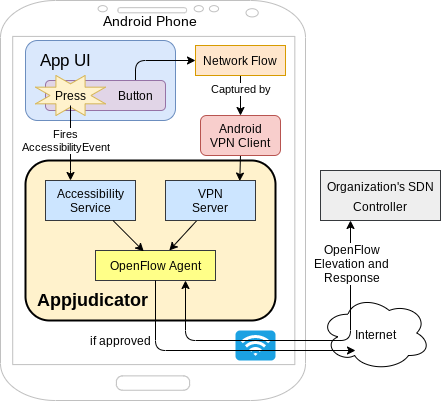
\includegraphics[width=.6\textwidth]{component-diagram.png}
    \caption{Diagram of component interactions.}
    \label{fig:component-diagram}
\end{wrapfigure}

The networking component of \textsc{Appjudicator} utilizes Android's built-in
API for redirecting network traffic, the VPN
Service~\cite{googledevelopers2020vpn}. We direct Android's built-in
VPN client to connect to a custom VPN server running on the Android device
itself. With the user's permission we can route all traffic through this VPN,
allowing us to capture all network flows entering and exiting the device. We implement a
low-level system for intercepting packets, inspecting their contents, and making
decisions on whether to forward the packets to their intended destination or
drop them.

Once activated, the VPN service runs in the background and receives packets from
the operating system through a file interface. An application can read from this
interface to get packets from the networking stack as raw byte arrays in the
same way it would read from any other file. Likewise we can write to the
interface like a file to send raw data to the network. \textsc{Appjudicator}
manages connections and forwards allowed packets to their remote destination
using Java sockets.

The VPN service provides network context that can be used by the SDN agent. For
example, the destination IP address, protocol, payload size, initiating
application, and full packet payload can all be used to enforce fine-grained SDN
rules.
% TODO write about how we get the initiating application in Implementation

Apps are likely to make some kinds of network requests independent of user
interaction, for example automatically fetching weather data from the Internet
every hour. To account for this we profile known-benign apps using tcpdump to
see what sort of requests they make independently over several hours with no
interaction, and record these flows in a default-allow list. Then, during normal
operation of the app if we receive a network flow that is not on this list
\textit{and} was not initiated by a user interaction we can investigate it
further.

\subsection{Accessibility Service}
\label{sec:approach-accessibility-service}

The user interface monitoring component is implemented as an Accessibility
Service, using Android's API for simulating and responding to user interaction
with the UI~\cite{googledevelopers2020}. This service runs in the background and
receives information from accessibility events asynchronously. These
accessibility events contain data about what action was performed (clicking,
swiping, entering text, \textit{etc}.) and what UI element was the target of the
action. This UI data is the key to the central idea of \textsc{Appjudicator}: it
lets us associate a network flow with the UI interaction that initiated it.

% Move this paragraph to background
Android accessibility services break the operating system's normally strong
sandboxing principles by their ability to read and interact with anything
displayed on the screen~\cite{kalysch2018}. For security reasons, Android
requires any accessibility service to be enabled manually by the user in the
settings app. But once the service is enabled it can run continuously in the
background, receiving accessibility events from almost any UI interaction in any
app.

\subsection{Software-defined Networking}
\label{sec:sdn-rule-cache}

We combine networking control from the VPN service with UI monitoring from the
accessibility service to create a context-enhanced SDN agent.
Figure~\ref{fig:component-diagram} shows how each of \textsc{Appjudicator}'s
components integrate with the other aspects of the phone environment. The app
acts as an OpenFlow-compatible agent while receiving UI interaction data from
the accessibility service and network flows from the VPN service. It enforces
policy on the device, forwarding, dropping, or elevating packets based on rules
received from the organization's OpenFlow controller server.

To do this, we implement a subset of the OpenFlow protocol, including logic for
caching rules from the controller server, inspecting packets, and enforcing
rules. The OpenFlow agent performs all the standard behavior of an SDN agent:
caching rules, forwarding packets according to rules, and elevating flows to the
controller server.

A flow's initiating UI interaction is determined by temporal association. When a
new flow is intercepted \textsc{Appjudicator} looks up the most recent UI
interactions from the same application to see if there was a likely initiator,
such as a button press, within the last two seconds. We send as much data about
any potential matches as we can fit into a packet-in OpenFlow message (see
Section~\ref{sec:openflow-protocol}) to the SDN controller when a flow is
elevated, to provide additional context.

\newpage

\section{Implementation}
\label{sec:implementation}

\textsc{Appjudicator} is a complex application with disparate components that
must run simultaneously and communicate with each other properly. The app can be
broadly broken down into three main components: the accessibility service, which
implements Android's \texttt{AccessibilityService}
API~\cite{googledevelopers2020}; the local VPN server, which implements
Android's \texttt{VpnService} API~\cite{googledevelopers2020vpn}; and the
host-based SDN agent, which implements a subset of the OpenFlow 1.0
standard~\cite{mckeown2008}.

The app is implemented using Kotlin, an object-oriented programming language
that is interoperable with Java and compiles to Java Virtual Machine bytecode.
This is Google's preferred language for Android development, and makes some
tasks like null-checking and concurrency easier than they would be in
Java~\cite{lardinois2019}.

\subsection{Accessibility Service}
\label{sec:implementation-accessibility-service}

Android's \texttt{AccessibilityService} API is designed for applications for
individuals with additional need for tools like screen readers and automated UI
navigators. By registering an accessibility service with the operating system,
we can be notified of changes in the UI state of other applications. These
changes are referred to as accessibility events, and are asynchronously
triggered by the Android operating system and delivered to the listening
accessibility service.

% TODO include details about the process of registering an accessibility service
% in code

\subsubsection{Accessibility Events}
\label{sec:accessibility-events}

An accessibility event represents a single state change in the user interface of
an app, such as a button being clicked, a view being swiped, or the focus
changing~\cite{accessibilityserviceguide}. An accessibility service can specify
the particular app packages and event types it wants to receive, but
\textsc{Appjudicator} registers for all all event types from all packages.

The accessibility event object contains some context about the UI interaction,
including the type of UI element, the type of interaction (\textit{e.g.} click,
swipe, long press), and descriptive text of the
element~\cite{accessibilityserviceguide}. Additional information about the UI
element that initiated the event can be retrieved with the
\texttt{AccessibilityEvent.getSource()} method. This method allows the app to
get information about the layout hierarchy, providing context about the
element's enclosing views and child elements. Because this context information
could potentially expose private user data the service must declare the
\texttt{canRetrieveWindowContent} attribute in its configuration XML file. With
this attribute set, Android will warn the user that the application can retrieve
the contents of the screen when it is enabled.

By default, the operating system only includes view objects it thinks are
important to accessibility with the accessibility event, but we can request
information about all views instead by passing the 
\texttt{FLAG\_INCLUDE\_NOT\_IMPORTANT\_VIEWS} flag to the accessibility
service~\cite{accessibilityserviceguide}.

These accessibility events are fired for almost every type of UI interaction,
including clicks, swipes, long presses, and even input from devices like virtual
or physical keyboard. However, events fired from apps that do not use Android's
UI libraries do not provide as much context. For example, we cannot get layout
hierarchy information from an app that renders its UI in OpenGL or some other
graphics platform~\cite{accessibilityserviceguide}.
%TODO get citation on this, maybe say that these types of events are rare

% TODO include an example of an accessibility event and layout hierarchy as a
% diagram or text. Show layout XML and the info we get side-by-side.

\subsubsection{Asynchronous Event Handling}
\label{sec:asynchronous-event-handling}

When an accessibility event is generated, the Android operating system passes
the generated object to the accessibility service's
\texttt{onAccessibilityEvent()} callback
asynchronously~\cite{googledevelopers2020}. The event handler does not block the
user interface because it runs on a different thread, which helps achieve the
our goal of adding minimal latency. However, this asynchronous processing also
means an app may continue generating accessibility events while an earlier event
is still being processed, so we must make sure to handle events efficiently.

\subsubsection{Identifying UI Elements}
\label{sec:identifying-ui-elements}

Accessibility events do not provide a unique identifier for UI elements, so we
implement a system inspired by Fazzini~\etal \cite{fazzini2017}. Android UI
elements, called views, may have an ID, but these are not guaranteed to be
unique or even present on every view. We use the initiating element's resource
ID and resort to a selector based on the element's position in the XML UI tree
if the ID is missing or non-unique. This allows us to precisely correlate a
network flow with the particular UI interaction that initiated it. These
selectors should also be relatively stable across multiple application launches
because they will not change as long as the app's UI structure remains constant.
Developers rarely make large structural changes to app interfaces because they
go against common human-computer interaction guidelines~\cite{norman2013}.

% TODO include an example.

\subsubsection{Permissions and Security}
\label{sec:accessibility-permissions}

\textsc{Appjudicator} declares a service that requests the
\texttt{BIND\_ACCESSIBILITY\_SERVICE} permission in the Android manifest file.
This declaration tells Android which class represents the service, and also
specifies another XML configuration file.  The file provides metadata about the
service, such as listing which types of accessibility events to subscribe to,
and providing a description of the service's purpose to be shown to the user
when it is enabled.

For security reasons an app cannot enable its own accessibility
service~\cite{kalysch2018}. To prevent malware from taking advantage of the
far-reaching permissions of accessibility services, a user must manually enable
the service in the system settings after being prompted with a dialogue box that
explains some of the risks involved. \textsc{Appjudicator} can only point the
user toward the settings page, the rest must be done manually. A user may have
any number of accessibility services running at a time, but they must be
individually manually enabled and each display a persistent notification
reminding the user that the service is still running in the background.

% TODO include screenshot of permissions warning

\subsection{VPN Service}
\label{sec:implementation-vpn-service}

In order to capture network context, we connect to a VPN server running locally
on the device using Android's \texttt{VpnService} API. We register a new VPN
connection using this API and prompt the user to connect to it. This routes all
the device's traffic through our service, which captures and logs packets before
forwarding them along to their destination.

The VPN service provides a \texttt{ParcelFileDescriptor} instance that can be
used to read and write packets from the interface's buffer~\cite{vpnguide}.
Normally, a VPN service would forward packets through a tunnel to a remote VPN
server, but \textsc{Appjudicator}'s VPN server runs locally on the device.
Packets are instead passed to processes running on other threads that log the
packets and forward them along to their destination.

% TODO write about how there's no encryption/decryption (get a citation)

\subsubsection{Deconstructing Flows}
\label{sec:deconstructing-flows}

Captured packets are parsed, logged, and reconstructed by the VPN service using
Pcap4J, a third-party Java IP packet library~\cite{kaito2016}. Source and
destination IP addresses are collected from the packet's IP header, along with
source and destination ports from the TCP or UDP header. \textsc{Appjudicator}
currently only supports IPv4, so any intercepted IPv6 packets are simply
dropped. Likewise, packets with unknown transport-layer protocols
(\textit{i.e.}, neither TCP nor UDP) are dropped.

% TODO explain how to link flows to PIDs and queue packets in a flow once I
% figure out how to do that

Packets are stored in a hash map indexed by the concatenation of source address,
source port, destination address, destination port, and protocol (either TCP or
UDP). Sequences of packets with identical values for each of these fields are
considered to be part of the same network flow. This system makes it easy to
look up all the packets belonging to a particular flow.

\subsubsection{Multithreading}
\label{sec:multithreading}

Network connections are performance-critical, so we need to ensure that the user
experience is not blocked waiting for \textsc{Appjudicator} to process network
requests. All network processing is performed off of the main thread using
Kotlin's concurrency framework. This allows the VPN service to have a minimal
impact on performance.

\subsubsection{Permissions and Security}
\label{sec:vpn-permissions}

For the VPN service to work, \textsc{Appjudicator} must request the
\texttt{INTERNET} permission and declare a service that requests the
\texttt{BIND\_VPN\_SERVICE} permission in the Android manifest. It must also
name a route to capture traffic from. We use \texttt{0.0.0.0/0} to capture all
IPv4 traffic, but this could be changed so the VPN is only used on traffic of a
particular interface or subnet.

After the app is installed, the VPN service can be started or stopped directly
from it. \textsc{Appjudicator} provides simple buttons to do this, or it can be
configured to connect to the VPN automatically on startup. The service can also
be stopped or disabled from Android's settings menu for security reasons.

% TODO add section about configuring the VPN. i.e. we always allow TCP traffic to
% the controller. The controller IP and port have to be inputted manually.

\subsection{Host-Based SDN}
\label{sec:host-based-sdn}

\textsc{Appjudicator} is designed to integrate with corporate SDN
infrastructure, so it needs to be able to communicate with an SDN controller
server. The OpenFlow switch specification, the de facto standard for
software-defined networking, describes a protocol for switch-controller
communication~\cite{openflowspec}. This specification is designed for large
network switches connected to potentially dozens of hosts, so implementing it on
a smartphone in Kotlin requires some special considerations.\footnote{See
Sections \ref{sec:software-defined-networking} and
\ref{sec:the-android-phone-as-an-sdn-agent} for a discussion of prior work in
host-based SDN agents on Android and other platforms.}

Large portions of the OpenFlow switch specification simply do not apply to
\textsc{Appjudicator}. For example, the app has no concept of Ethernet frames
and only one ``physical port'' in the sense that it is a switch for only one
host.

% TODO talk about potentially connecting to multiple controllers in the future

\subsubsection{SDN Rule Cache}
\label{sec:implementation-sdn-rule-cache}

\textsc{Appjudicator} implements a subset of the OpenFlow standard as a
host-based SDN agent. It acts in conjunction with a central SDN controller
server, and caches packet-forwarding rules from the server on the device. If a
particular network flow seems suspicious, or the SDN agent does not have a rule
for it, the entire packet can be elevated to the controller along with
contextual information such as details about any recent UI interactions as part
of a ``packet in'' message. \textsc{Appjudicator} will continue forwarding,
blocking, or elevating packets in other flows while waiting for a response from
the SDN controller. The controller makes a decision based on the network and UI
context and sends back a ``packet out'' response describing what to do with the
flow.

\subsubsection{OpenFlow Protocol}
\label{sec:openflow-protocol}

The OpenFlow Switch Specification describes a protocol for SDN agents to connect
to a controller and exchange messages. \textsc{Appjudicator} implements the
minimum allowable subset of this specification. All OpenFlow messages are sent
over TCP in OpenFlow packets. These packets have a simple 8-byte header that
describes the OpenFlow version, the type of the message, the total length of the
packet, and transaction ID (see Figure~\ref{fig:openflow-header}). Replies to an
OpenFlow message have the same transaction ID as the request.

\begin{figure}[h]
    \centering
    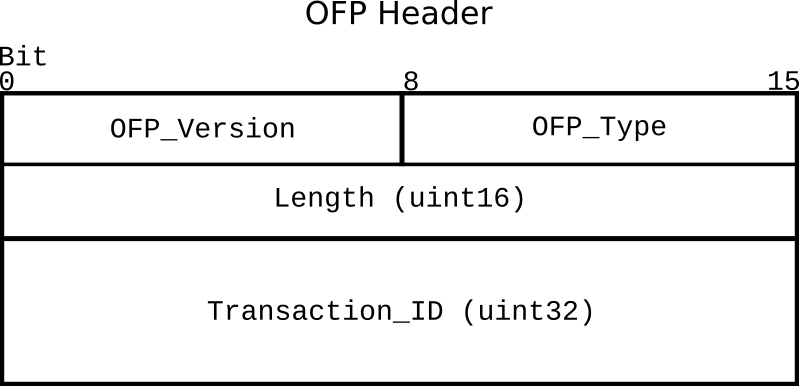
\includegraphics[width=.6\textwidth]{openflow-header.png}
    \caption{Fields of an OpenFlow packet header.}
    \label{fig:openflow-header}
\end{figure}

When the app is launched it opens a new TCP connection to a user-configurable IP
address or host name that runs the controller server. The controller and switch
each send a message of type \texttt{OFPT\_HELLO} to initiate the connection. The
controller then queries the switch to see what capabilities and features it
supports with a \texttt{OFPT\_FEATURES\_REQUEST}.  \textsc{Appjudicator} replies
with a message explaining that it has one physical port (the phone itself) and
only supports two packet actions: forward and drop.  At this point the
connection is fully established, and the controller and agent can both send
messages back and forth. Figure~\ref{fig:openflow-handshake} shows this process.

% TODO talk about how we only support a subset of normal flow table entries

\begin{wrapfigure}{R}{0.4\textwidth}
	\centering
	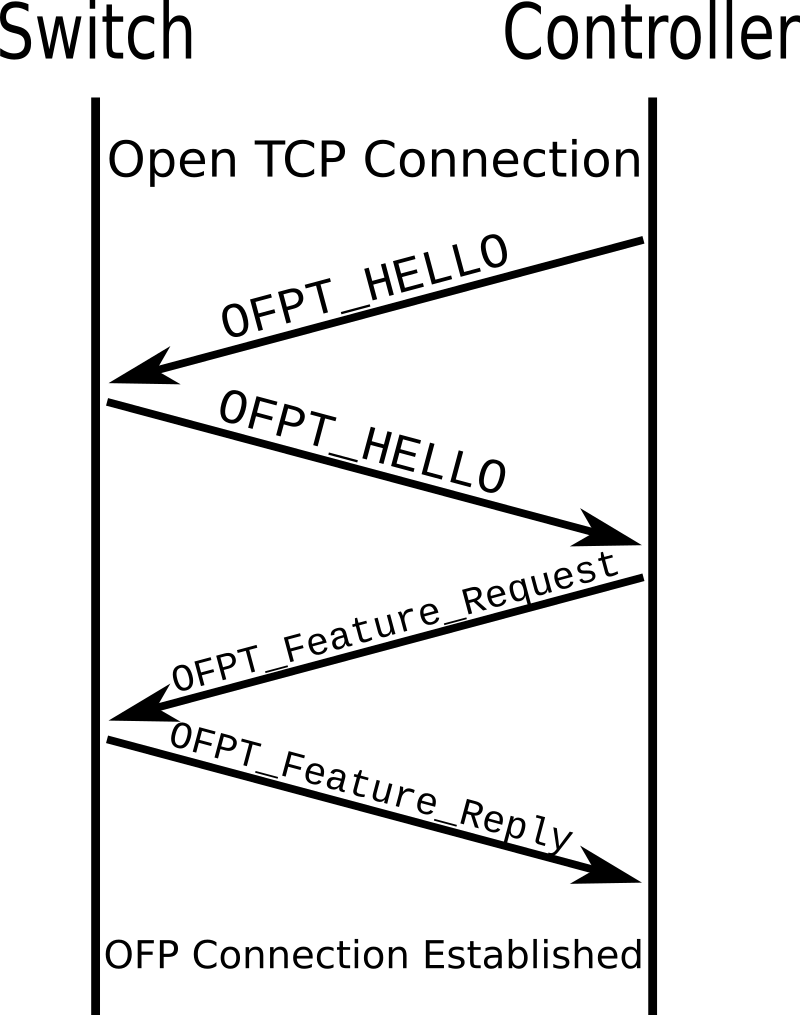
\includegraphics[width=0.4\textwidth]{openflow-handshake.png}
    \caption{OpenFlow handshake diagram.}
    \label{fig:openflow-handshake}
\end{wrapfigure}

% TODO add more about switch-initiated messages (packet-in and packet-out)

\subsubsection{Associating Network Flows with Context}
\label{sec:associating-network-flows-with-context}

\textit{[Details of this section may change.]}

When the SDN agent intercepts a new flow to a previously unknown domain, it
tries to associate it with UI context. The app looks up any accessibility events
that occurred in the two seconds before the flow was initiated. If there is no
likely initiator of the network flow (such as a button press) within the two
prior seconds the flow is considered non-user-initiated. The SDN agent includes
information about these UI events, including the event type and view hierarchy
(see Section~\ref{sec:identifying-ui-elements}) with the packet as it is
elevated to the controller. This UI context should allow for more powerful and
fine-grained SDN rules.

% TODO add more info here, stuff about getting PIDs

\subsubsection{Default-Allow Flows}
\label{sec:default-allow-flows}

Our system must account for non-user-initiated flows that occur as part of the
normal operation of the device. To do this, we profile the Android operating
system and common applications in advance.  While running in calibration mode,
\textsc{Appjudicator} adds the IP address and ports of all non-user-initiated
requests to a default-allow map. Then later, while operating normally, the app
will not question flows to these pairs of IP address and ports even if they are
not user-initiated.

% TODO add more info here

% TODO what to do when controller is unavailable

\newpage

\section{Evaluation and Results}
\label{sec:evaluation-and-results}

% ----- BEGIN PROPOSAL VERSION -----

To assess the functionality and efficiency of the system, we will conduct a series of experiments using a subset of the most popular apps in the Google Play store to see what amount of overhead is added by \textsc{Appjudicator} and whether it can distinguish user-generated from automated flows. In particular, we will measure the additional CPU, memory, and storage usage, as well as the amount of latency introduced by our system. We will perform a standard set of network operations that simulate real life use cases in various apps while our system is enabled and disabled. We will use Android's hardware monitors and traffic capture apps to measure added overhead, and average them across several trials. These tests can be automated with testing frameworks such as Google's UI Automator~\cite{uiautomator2020}.

We expect the added overhead of the VPN and SDN services to be similar to existing Android firewall solutions. Preliminary work implementing a host-based SDN agent for Microsoft Windows introduced a maximum of six milliseconds of delay in 96\% of network flows~\cite{chuluundorj2019}. While we expect the Java Virtual Machine implementation on Android to have more overhead than the relatively efficient Windows version, we still aim for a maximum added latency of less than one frame time on a 60 Hz display, which is about 16 milliseconds. This level of latency should be imperceptible to users.

We will also test how effective the system is at differentiating user-generated network flows from automated ones. On several popular apps from the Google Play store we will first create a default-allow list of automated network requests generated by the apps during normal operation. Then we will initiate new network requests both with and without user interaction to see if \textsc{Appjudicator} can distinguish non-user-initiated flows.

% ----- END PROPOSAL VERSION -----

\subsection{Testing Procedures}
\label{sec:testing-procedures}

% Use Android virtual machines to perform tests
% Use Google’s UI Automator to simulate user interaction

\subsection{Measuring Overhead}
\label{sec:measuring-overhead}

% Use top 20 most downloaded Google Play apps
% Simulate real use cases with Appjudicator enabled and disabled
% Measure CPU load, battery usage, average RTT and average across several trials
% Include a nice graph

\subsection{Differentiating User-generated Flows}
\label{sec:differentiating-user-generated-flows}

% Use UI Automator to simulate real clicks, also find other apps that make background requests automatically
% Log whether each flow was user-generated, default-allowed, or automated
% What percentage of those flows were classified successfully?

\newpage

\section{Conclusion}
\label{sec:conclusion}

\lipsum

\newpage


\label{sec:references}
%\printbibliography
\bibliographystyle{IEEEtranS}
\bibliography{references}

\end{document}
